\section{Results}

\begin{figure}[H]
	\centering
	
\includegraphics[width=0.88\textwidth]{content/plots/1.jpg}
	\caption{Detector-Scan with fitted Gaussian and marked half maximum positions.}
	\label{fig:detector-scan}
\end{figure}

\begin{figure}[H]
	\centering
	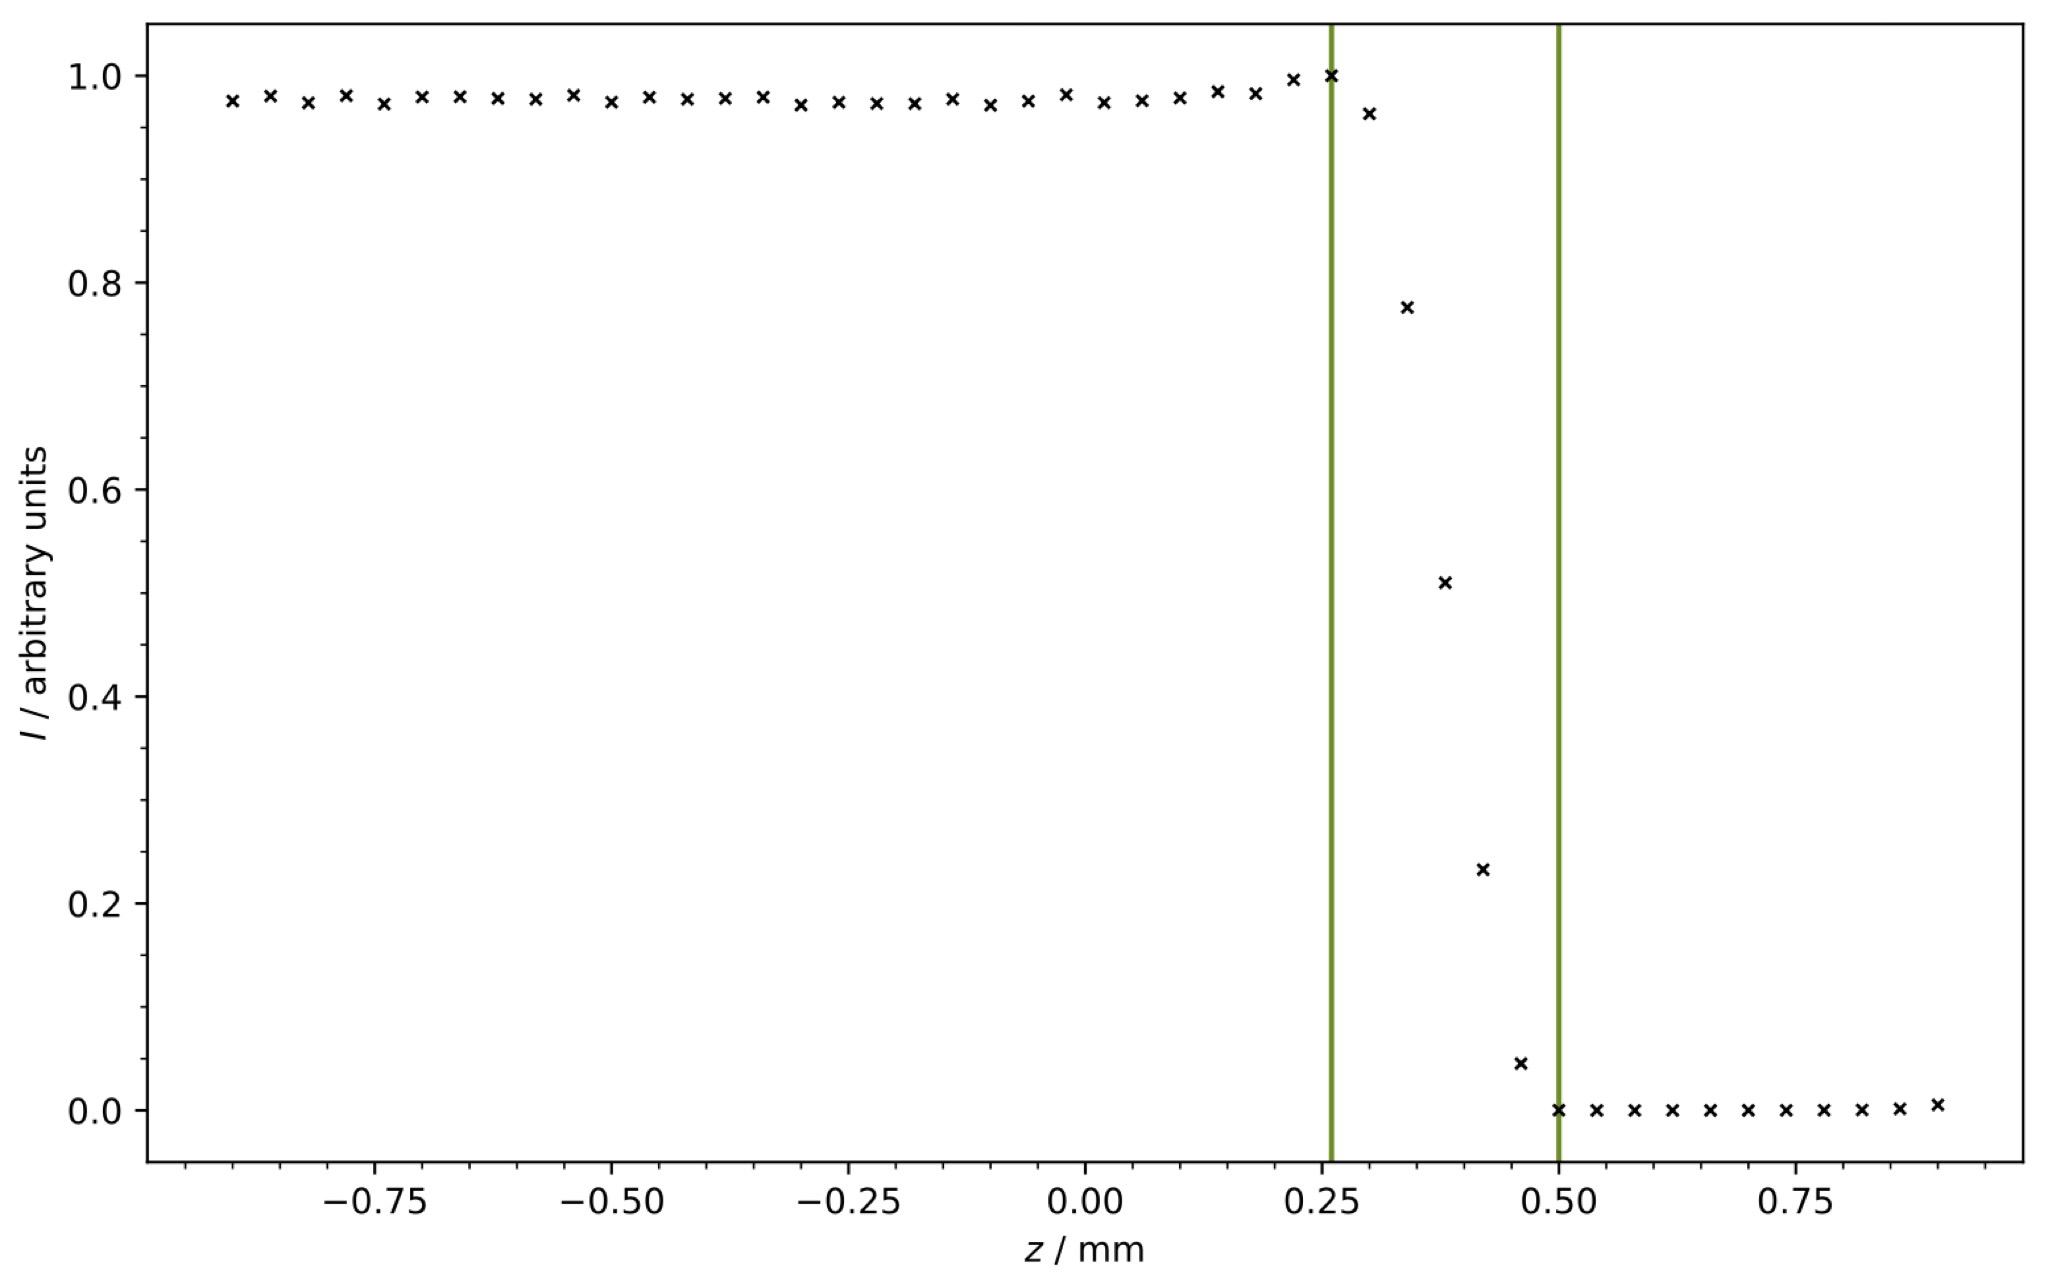
\includegraphics[width=0.88\textwidth]{content/plots/2.jpg}
	\caption{Z-Scan with indicated beam width.}
	\label{fig:z-scan}
\end{figure}

\begin{figure}[H]
	\centering
	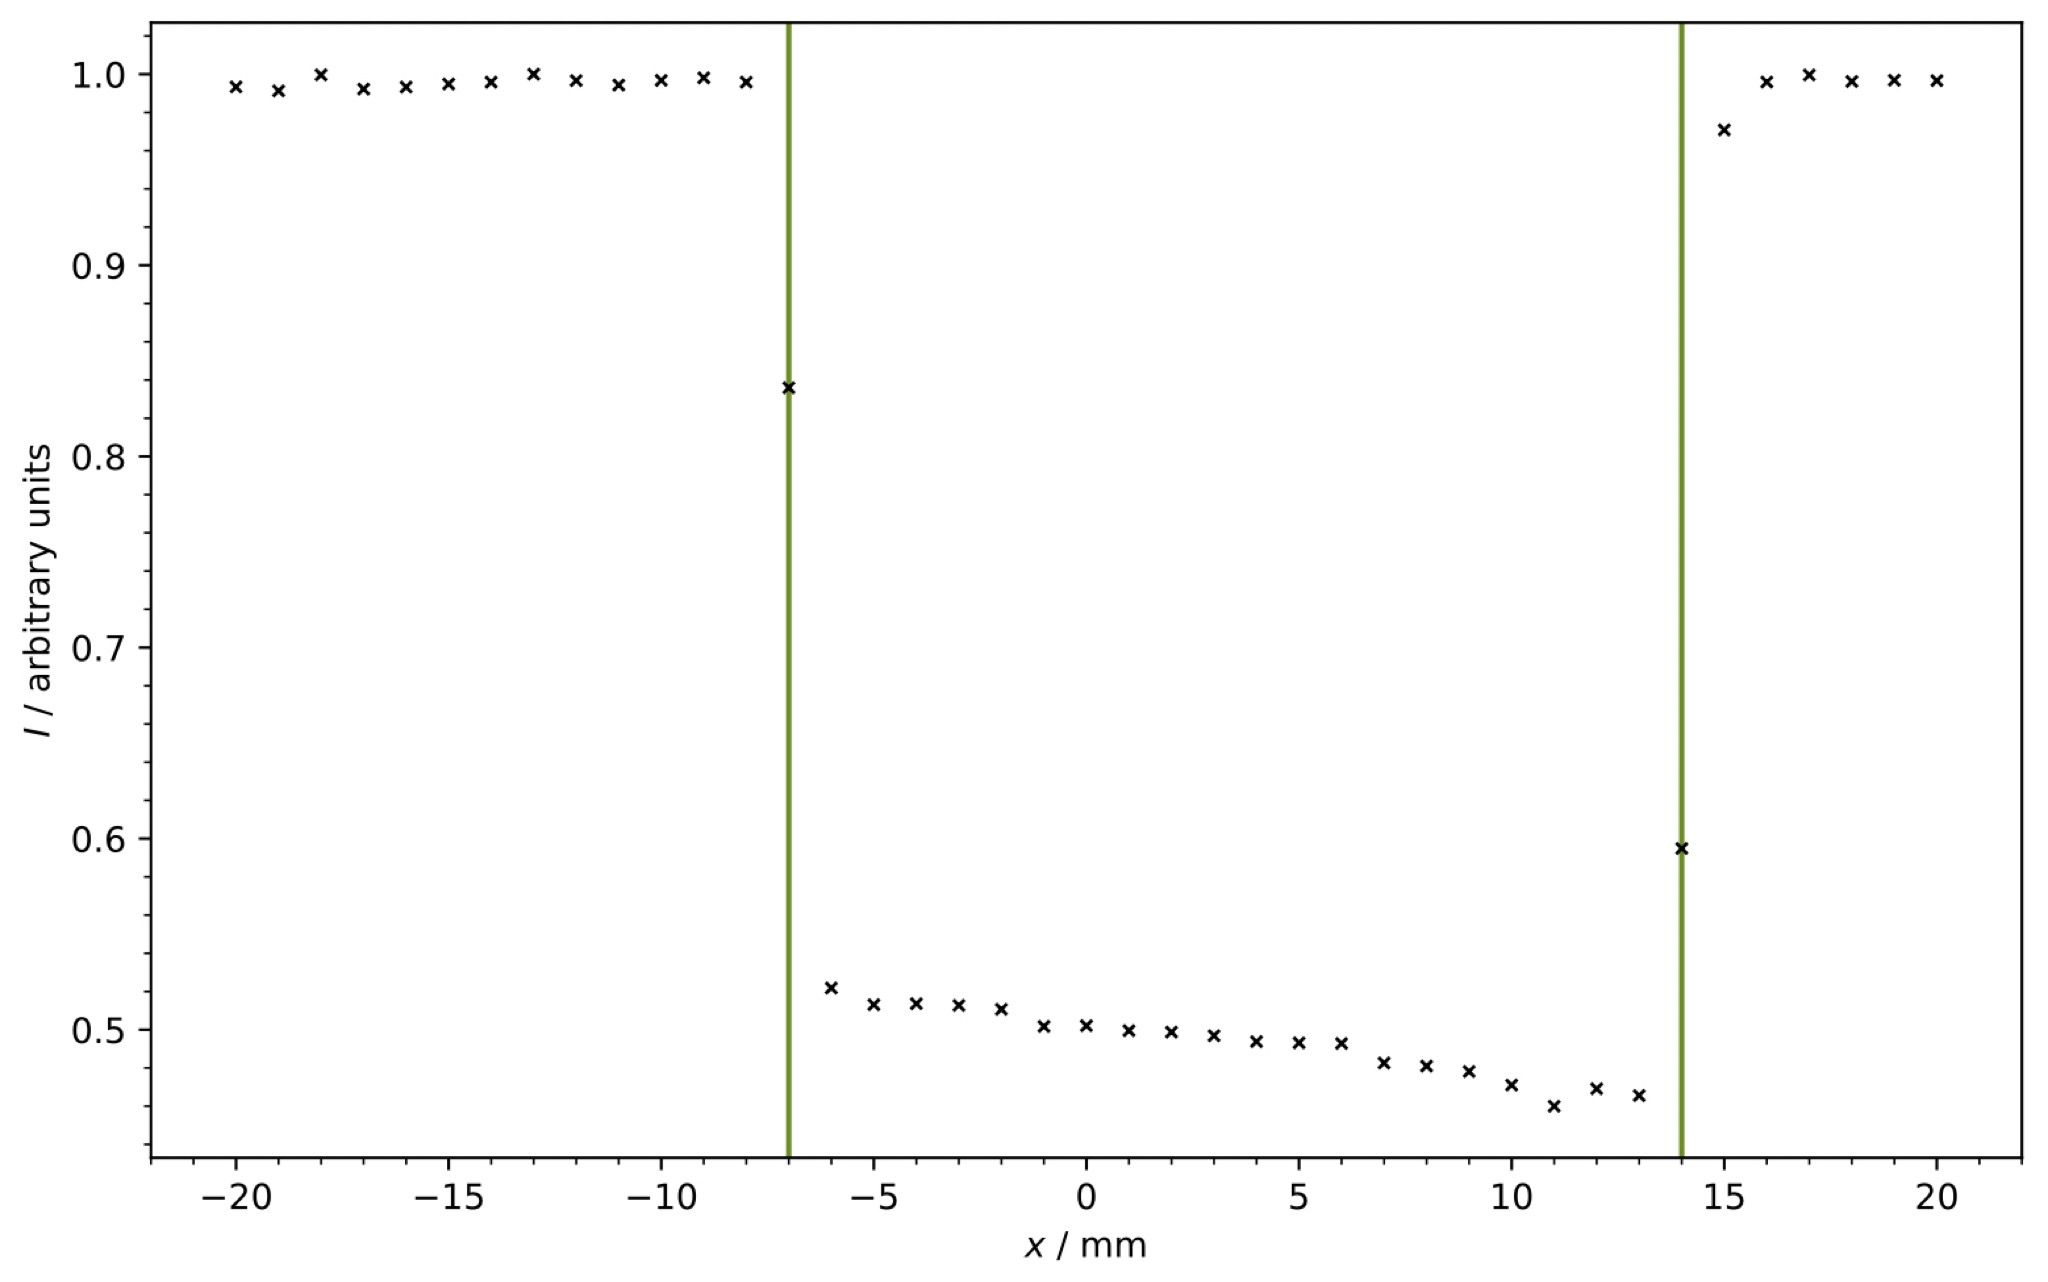
\includegraphics[width=0.88\textwidth]{content/plots/3.jpg}
	\caption{X-Scan with indicated sample size.}
	\label{fig:x-scan}
\end{figure}

\begin{figure}[H]
	\centering
	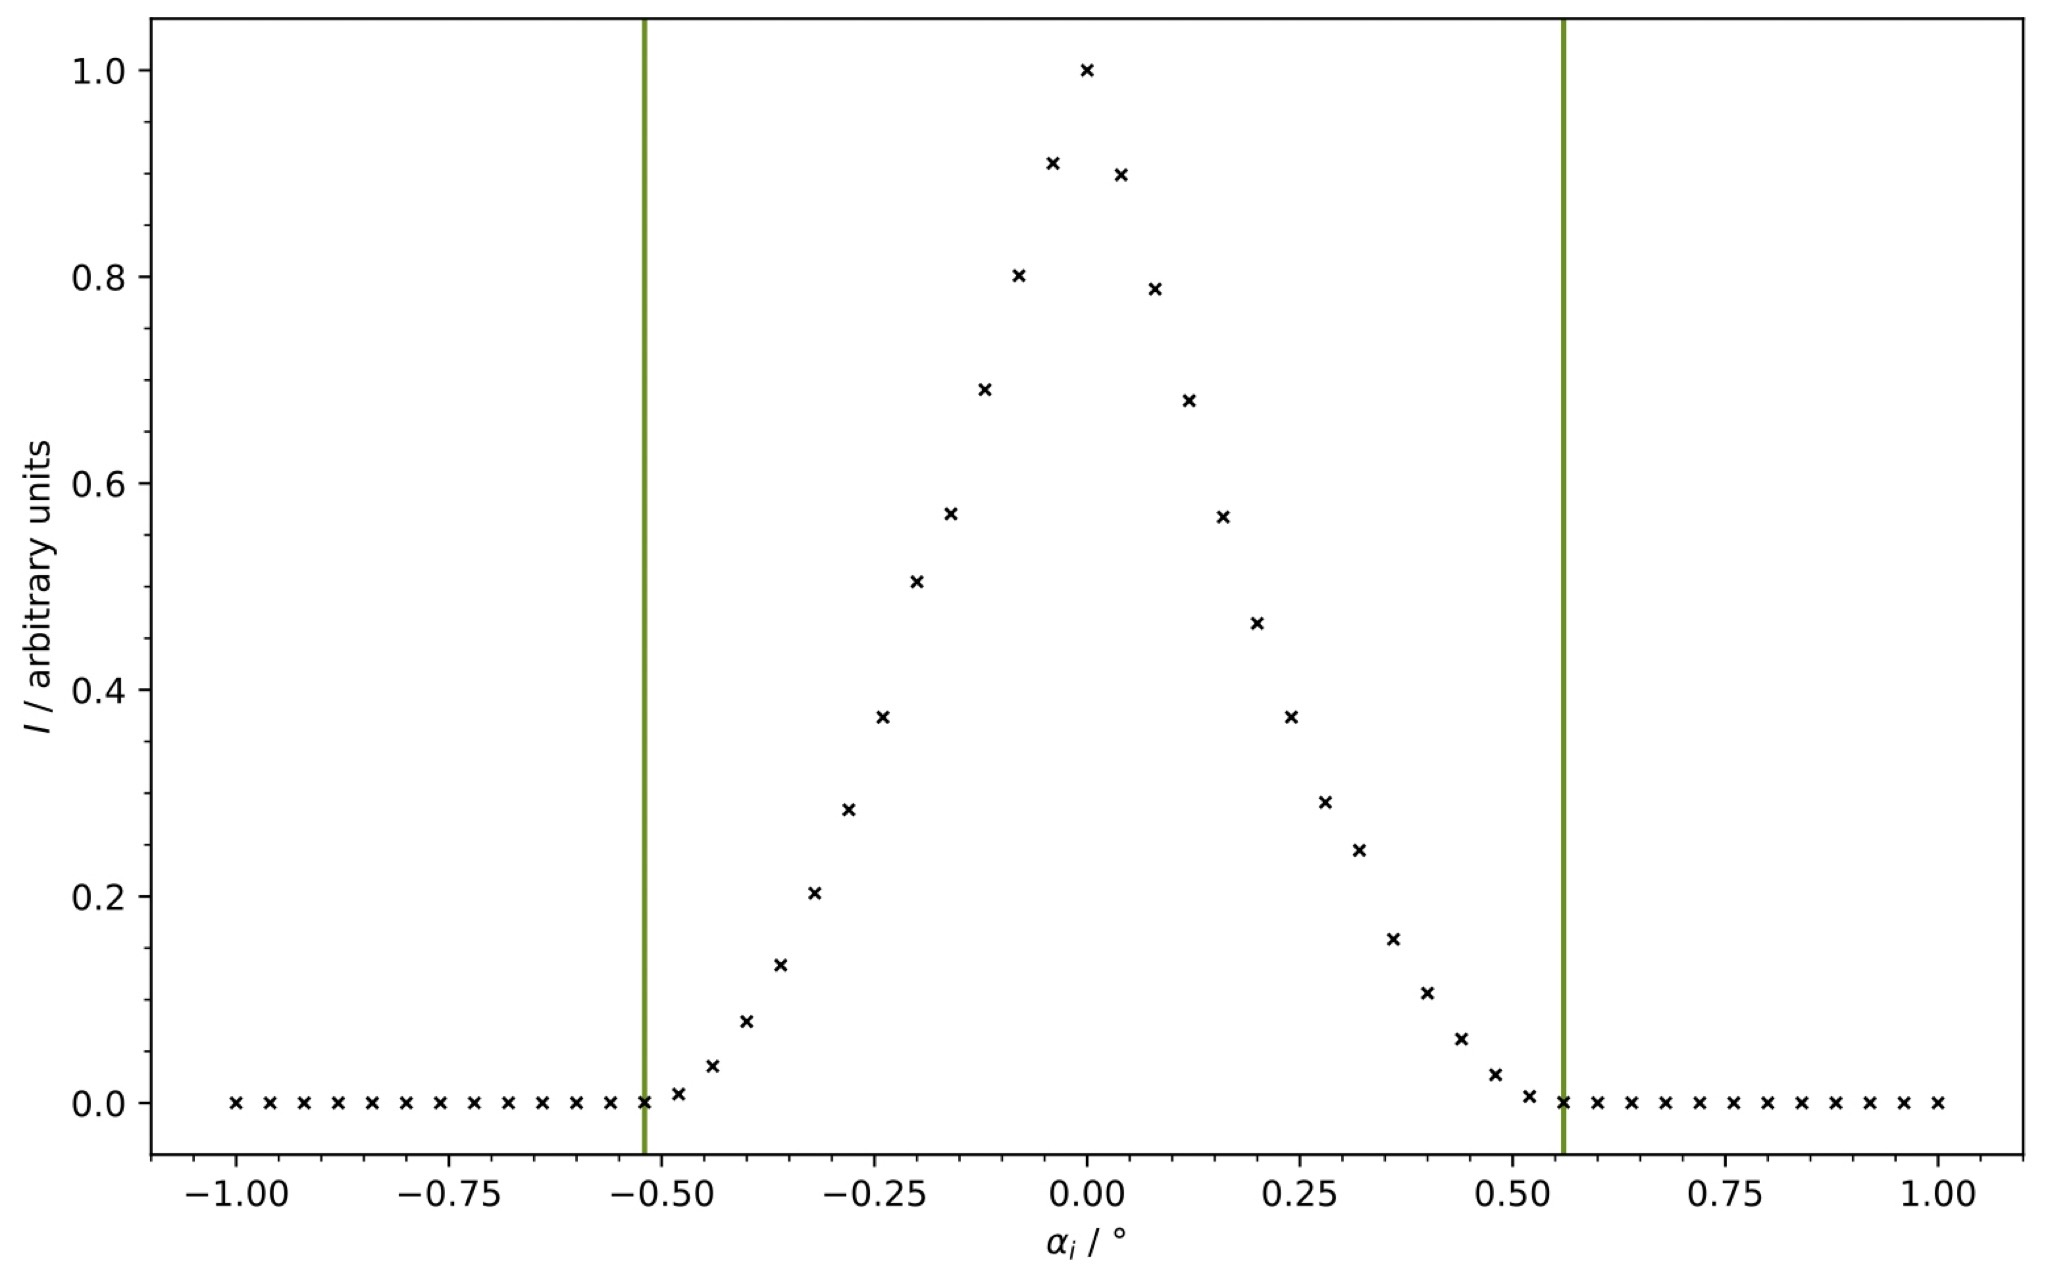
\includegraphics[width=0.88\textwidth]{content/plots/4.jpg}
	\caption{Rocking-Curve with geometry angles.}
	\label{fig:rocking-curve}
\end{figure}

\begin{figure}[H]
	\centering
	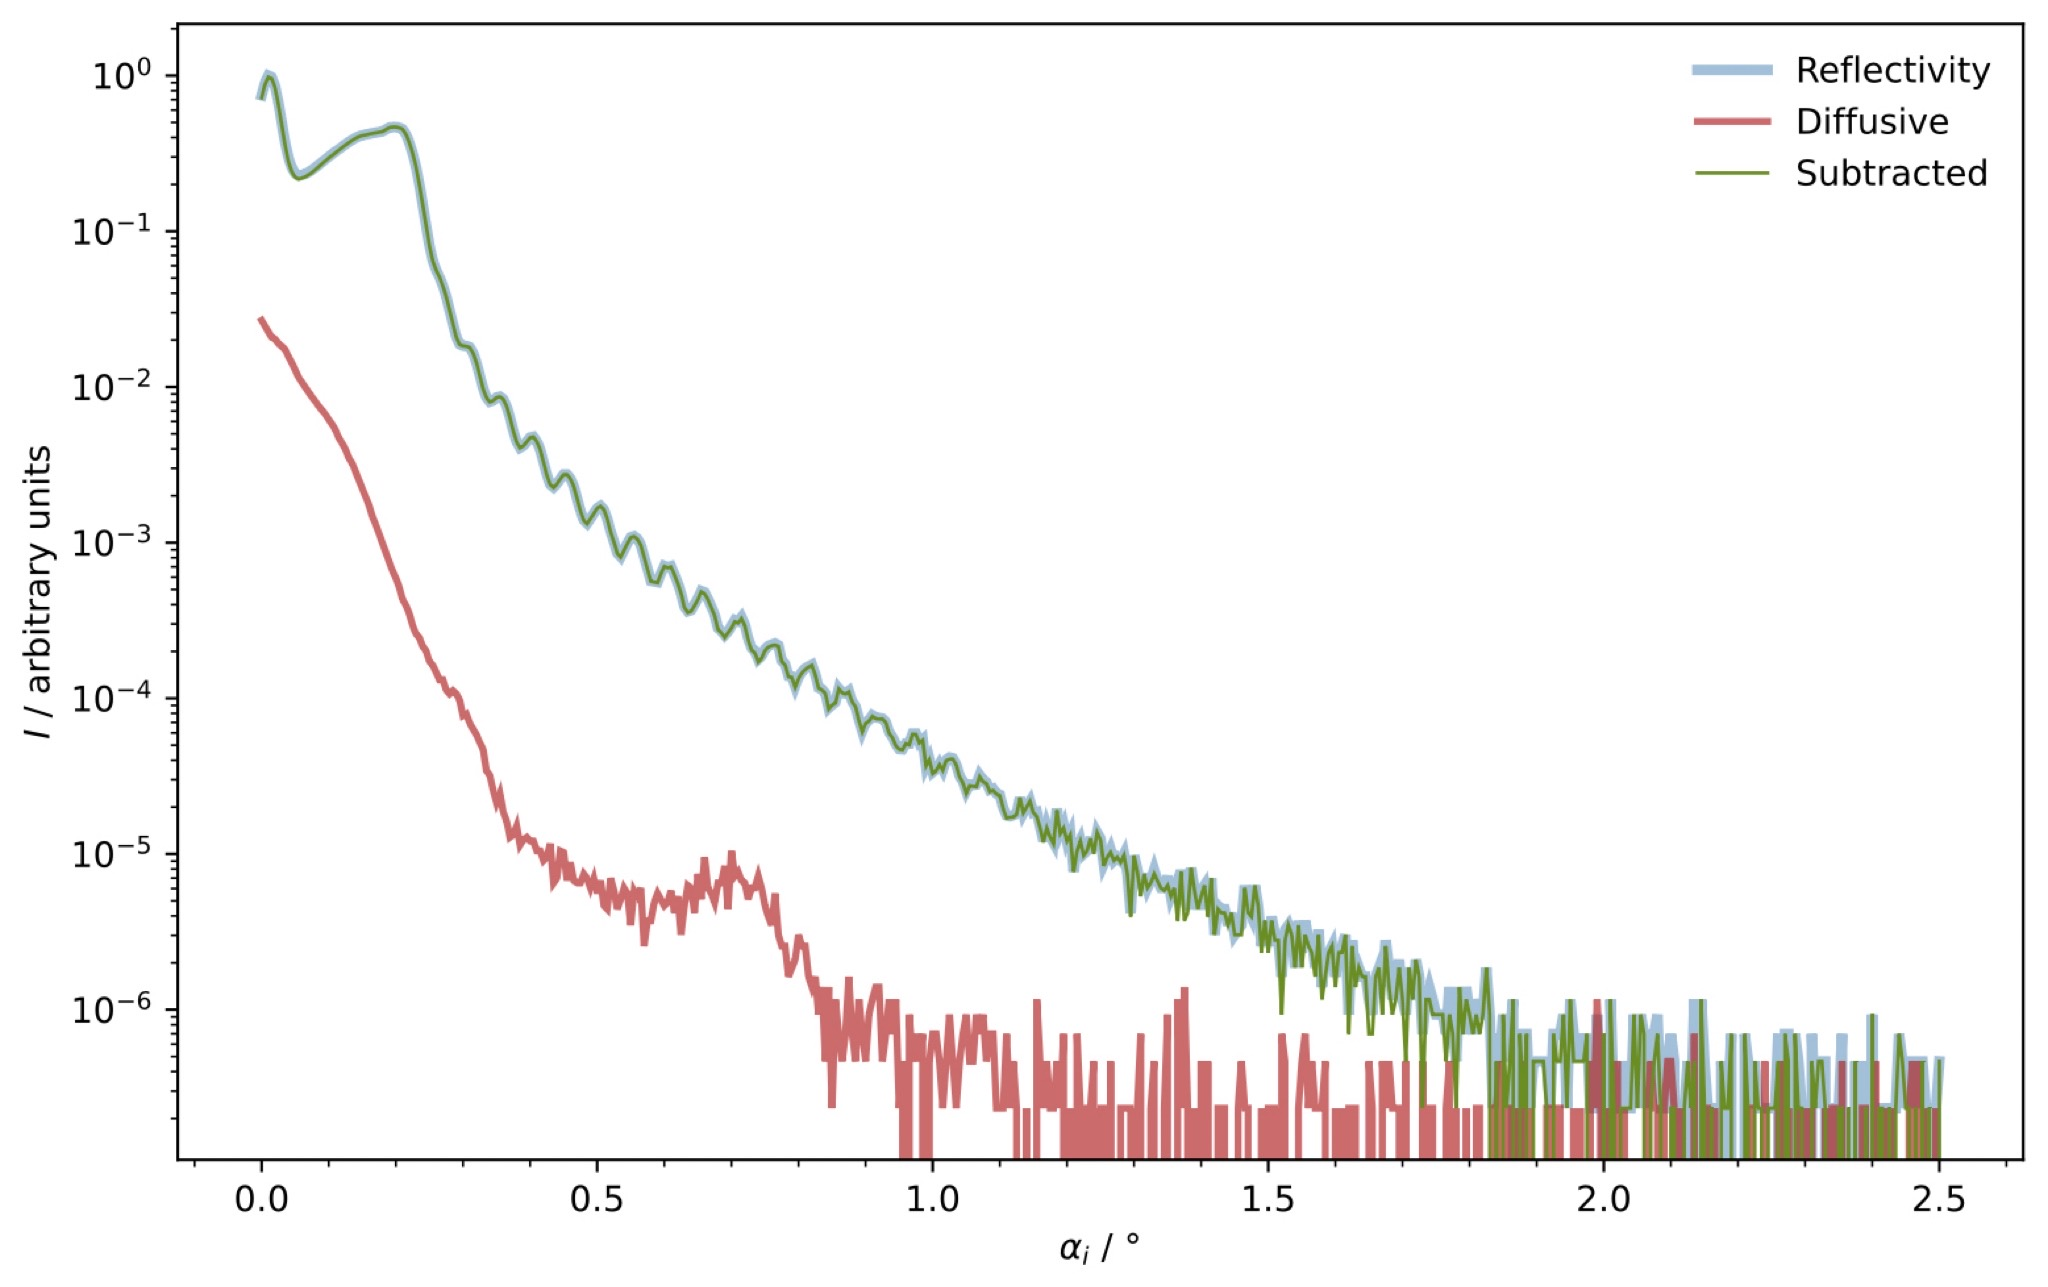
\includegraphics[width=0.88\textwidth]{content/plots/5.jpg}
	\caption{Intensity curves for reflectivity and diffusive background.}
	\label{fig:reflex-diffuse}
\end{figure}

\begin{figure}[H]
	\centering
	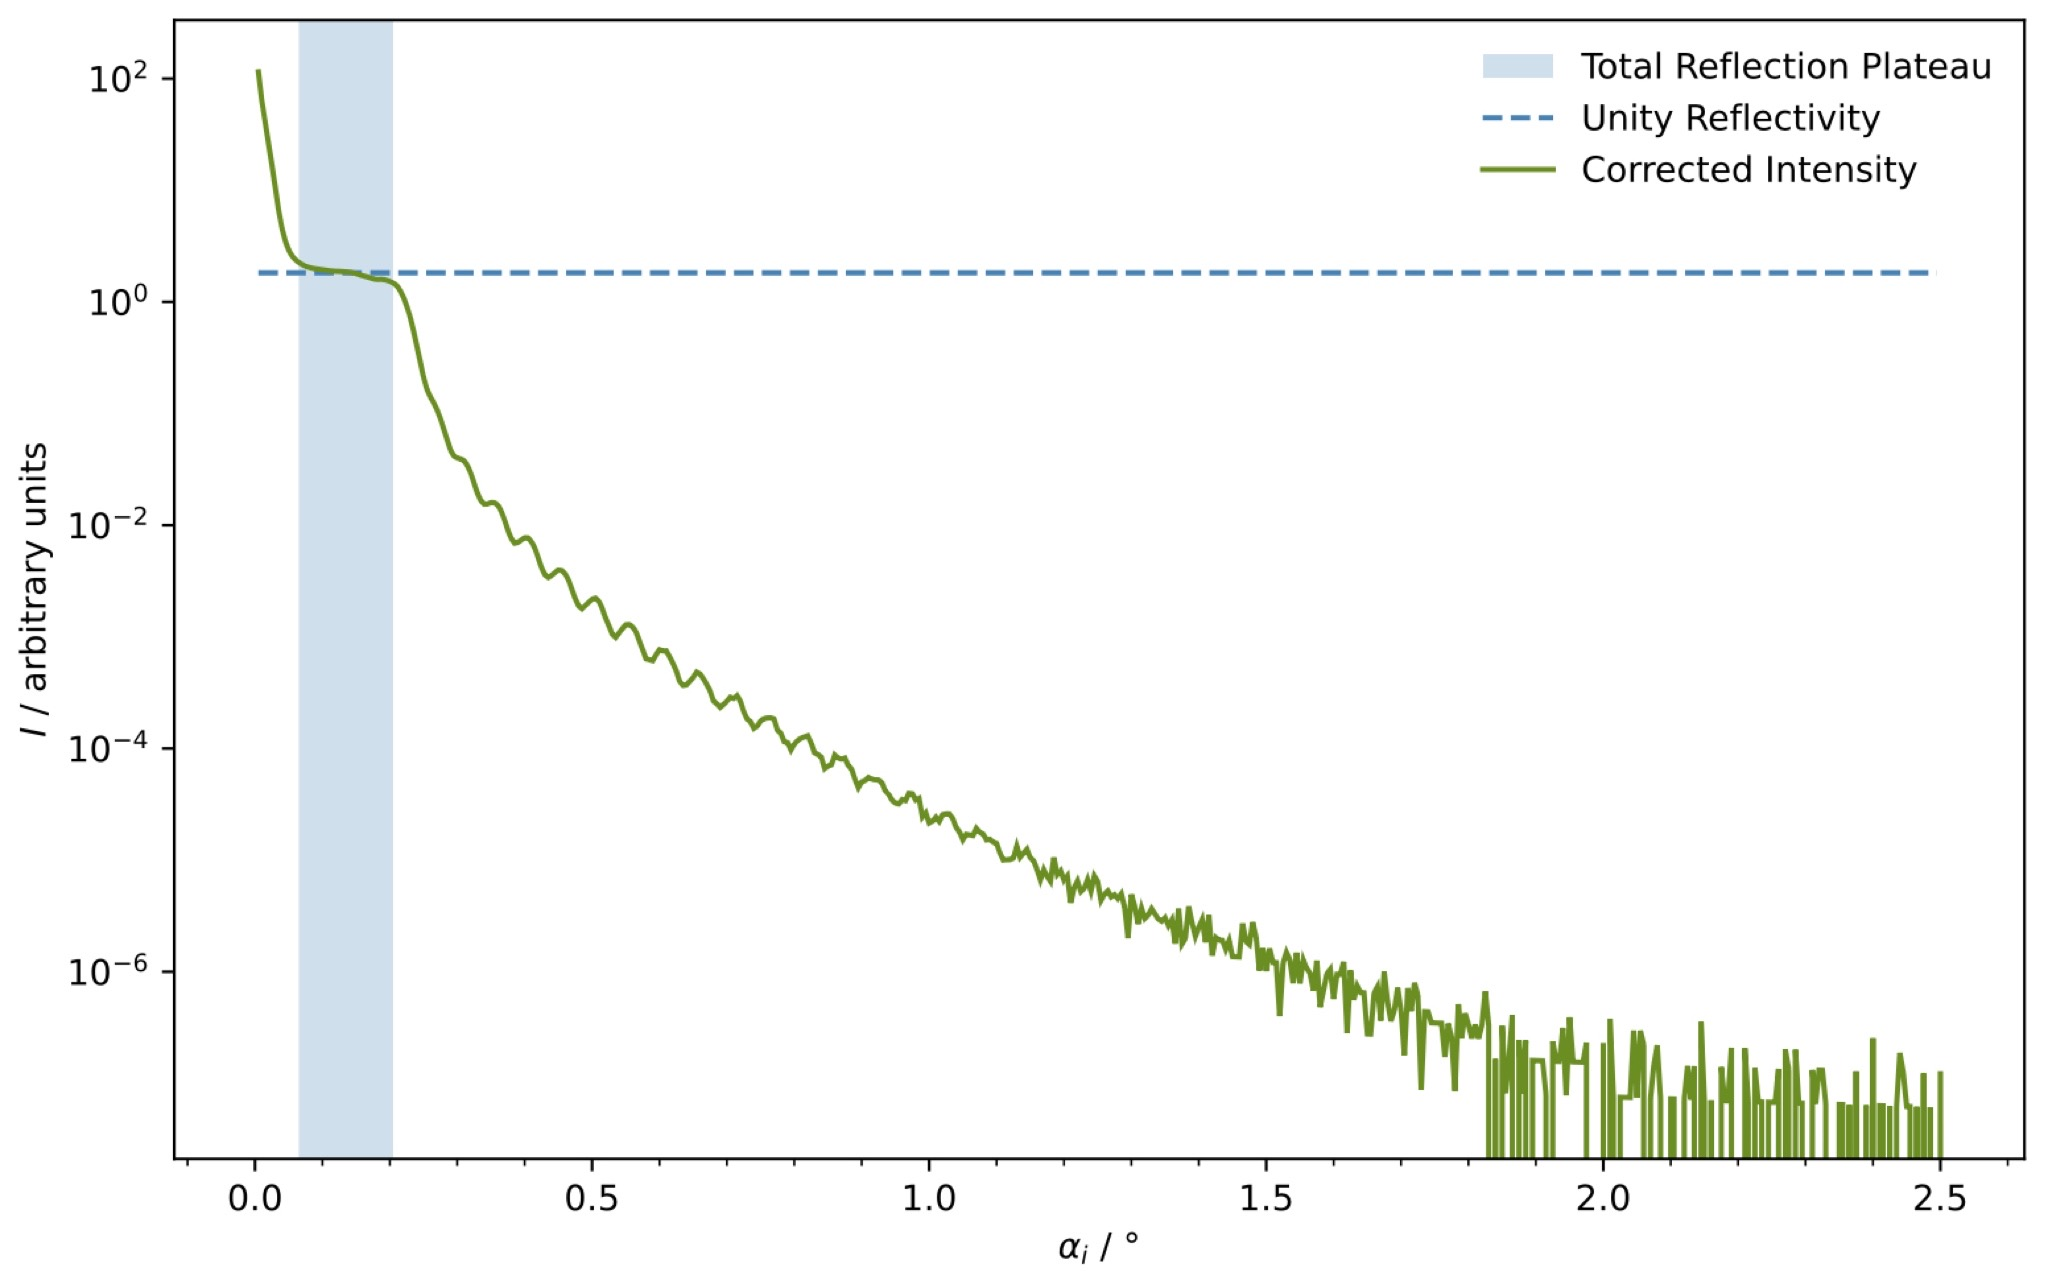
\includegraphics[width=0.88\textwidth]{content/plots/6.jpg}
	\caption{Intensity after geometry factor correction and region of total reflection.}
	\label{fig:geom-corr}
\end{figure}

\begin{figure}[H]
	\centering
	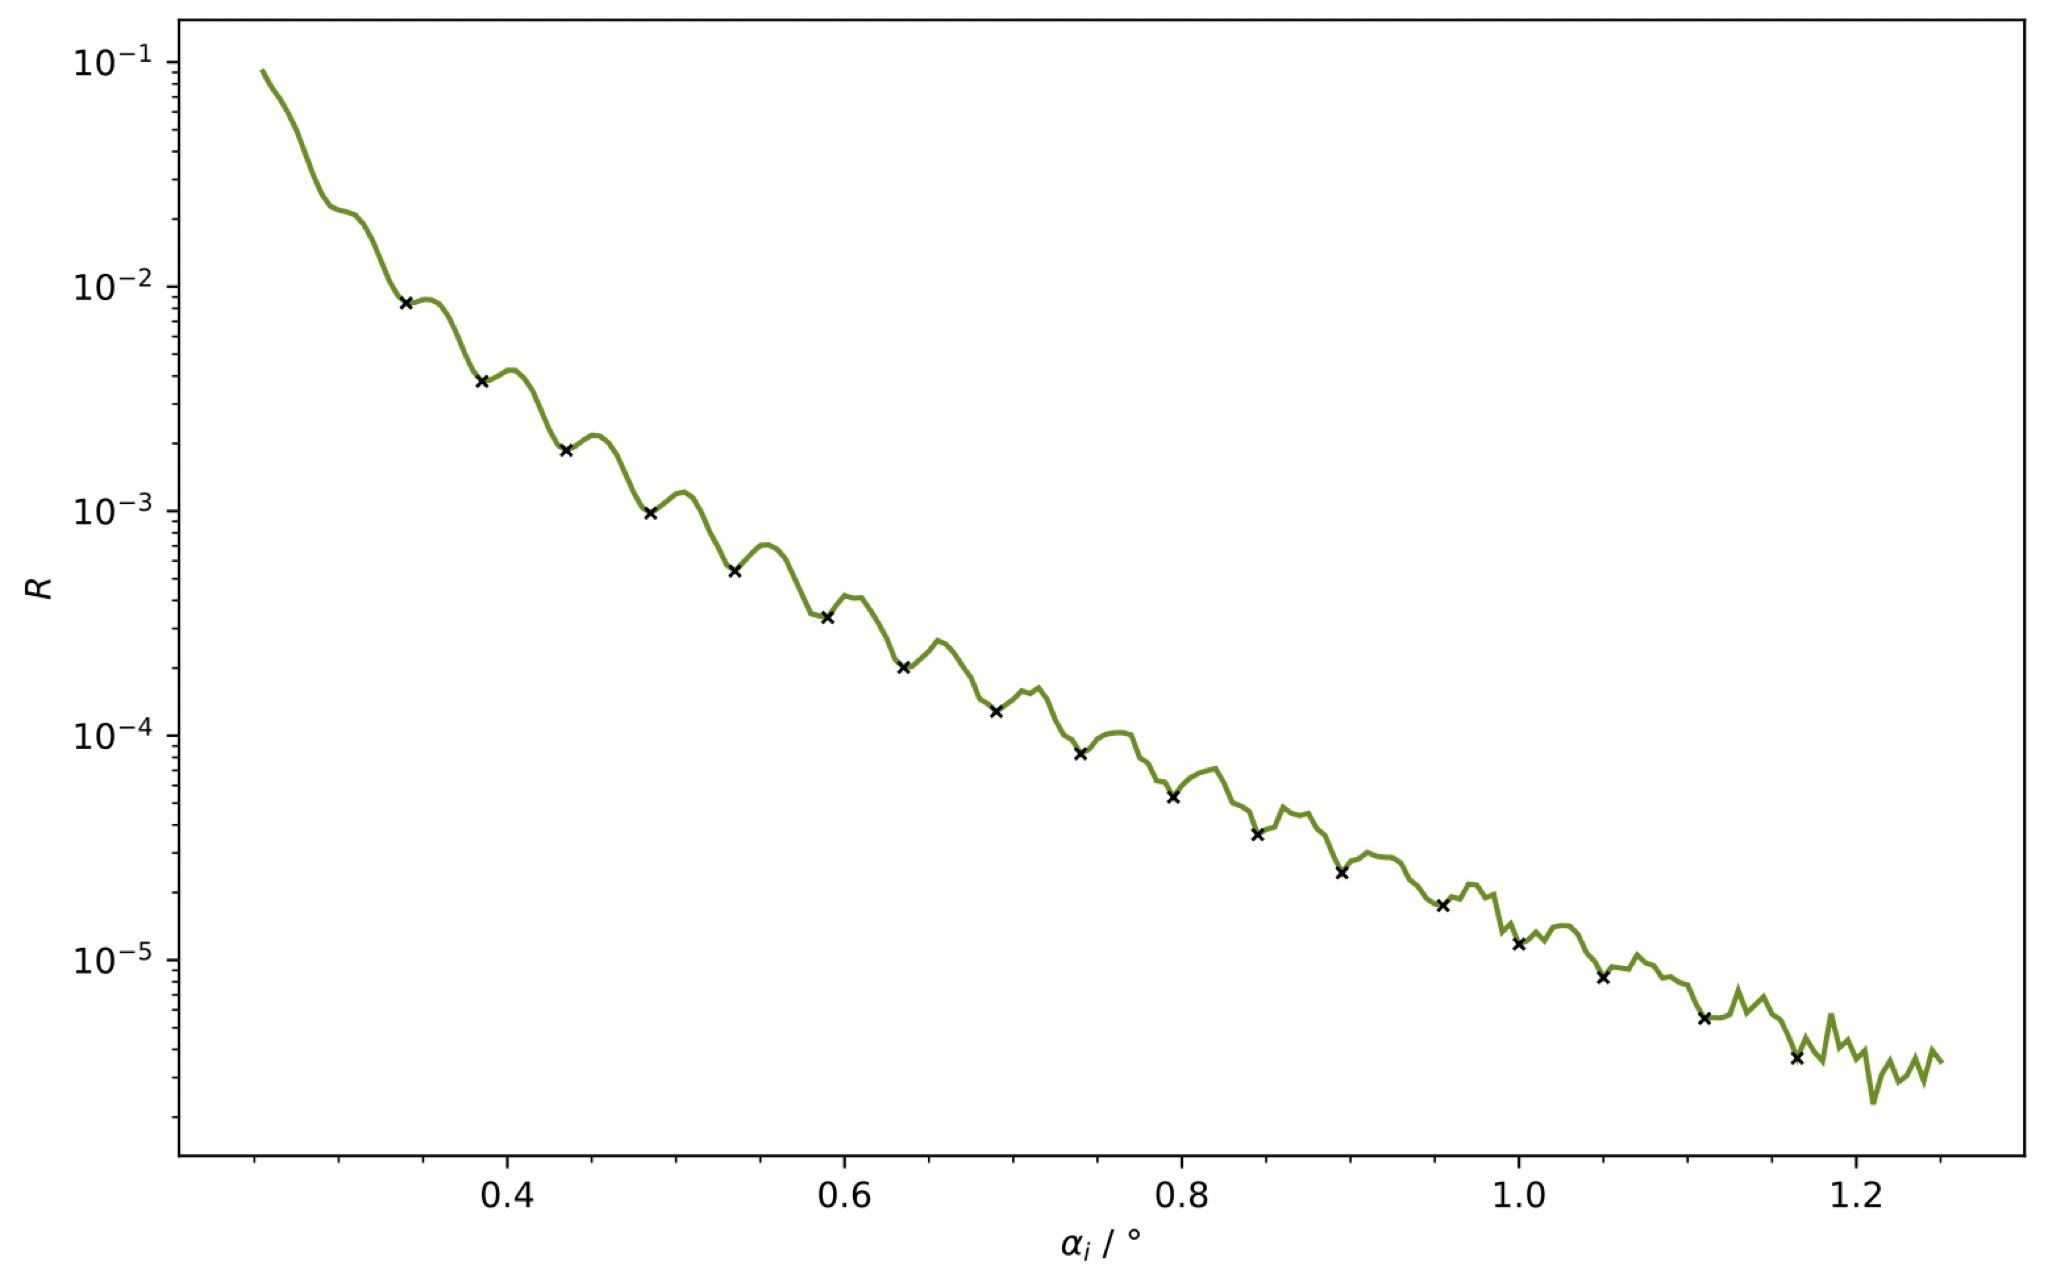
\includegraphics[width=0.88\textwidth]{content/plots/7.jpg}
	\caption{Detailed reflectivity curve with Kiessig oscillation minima.}
	\label{fig:kiessig-peaks}
\end{figure}

\begin{figure}[H]
	\centering
	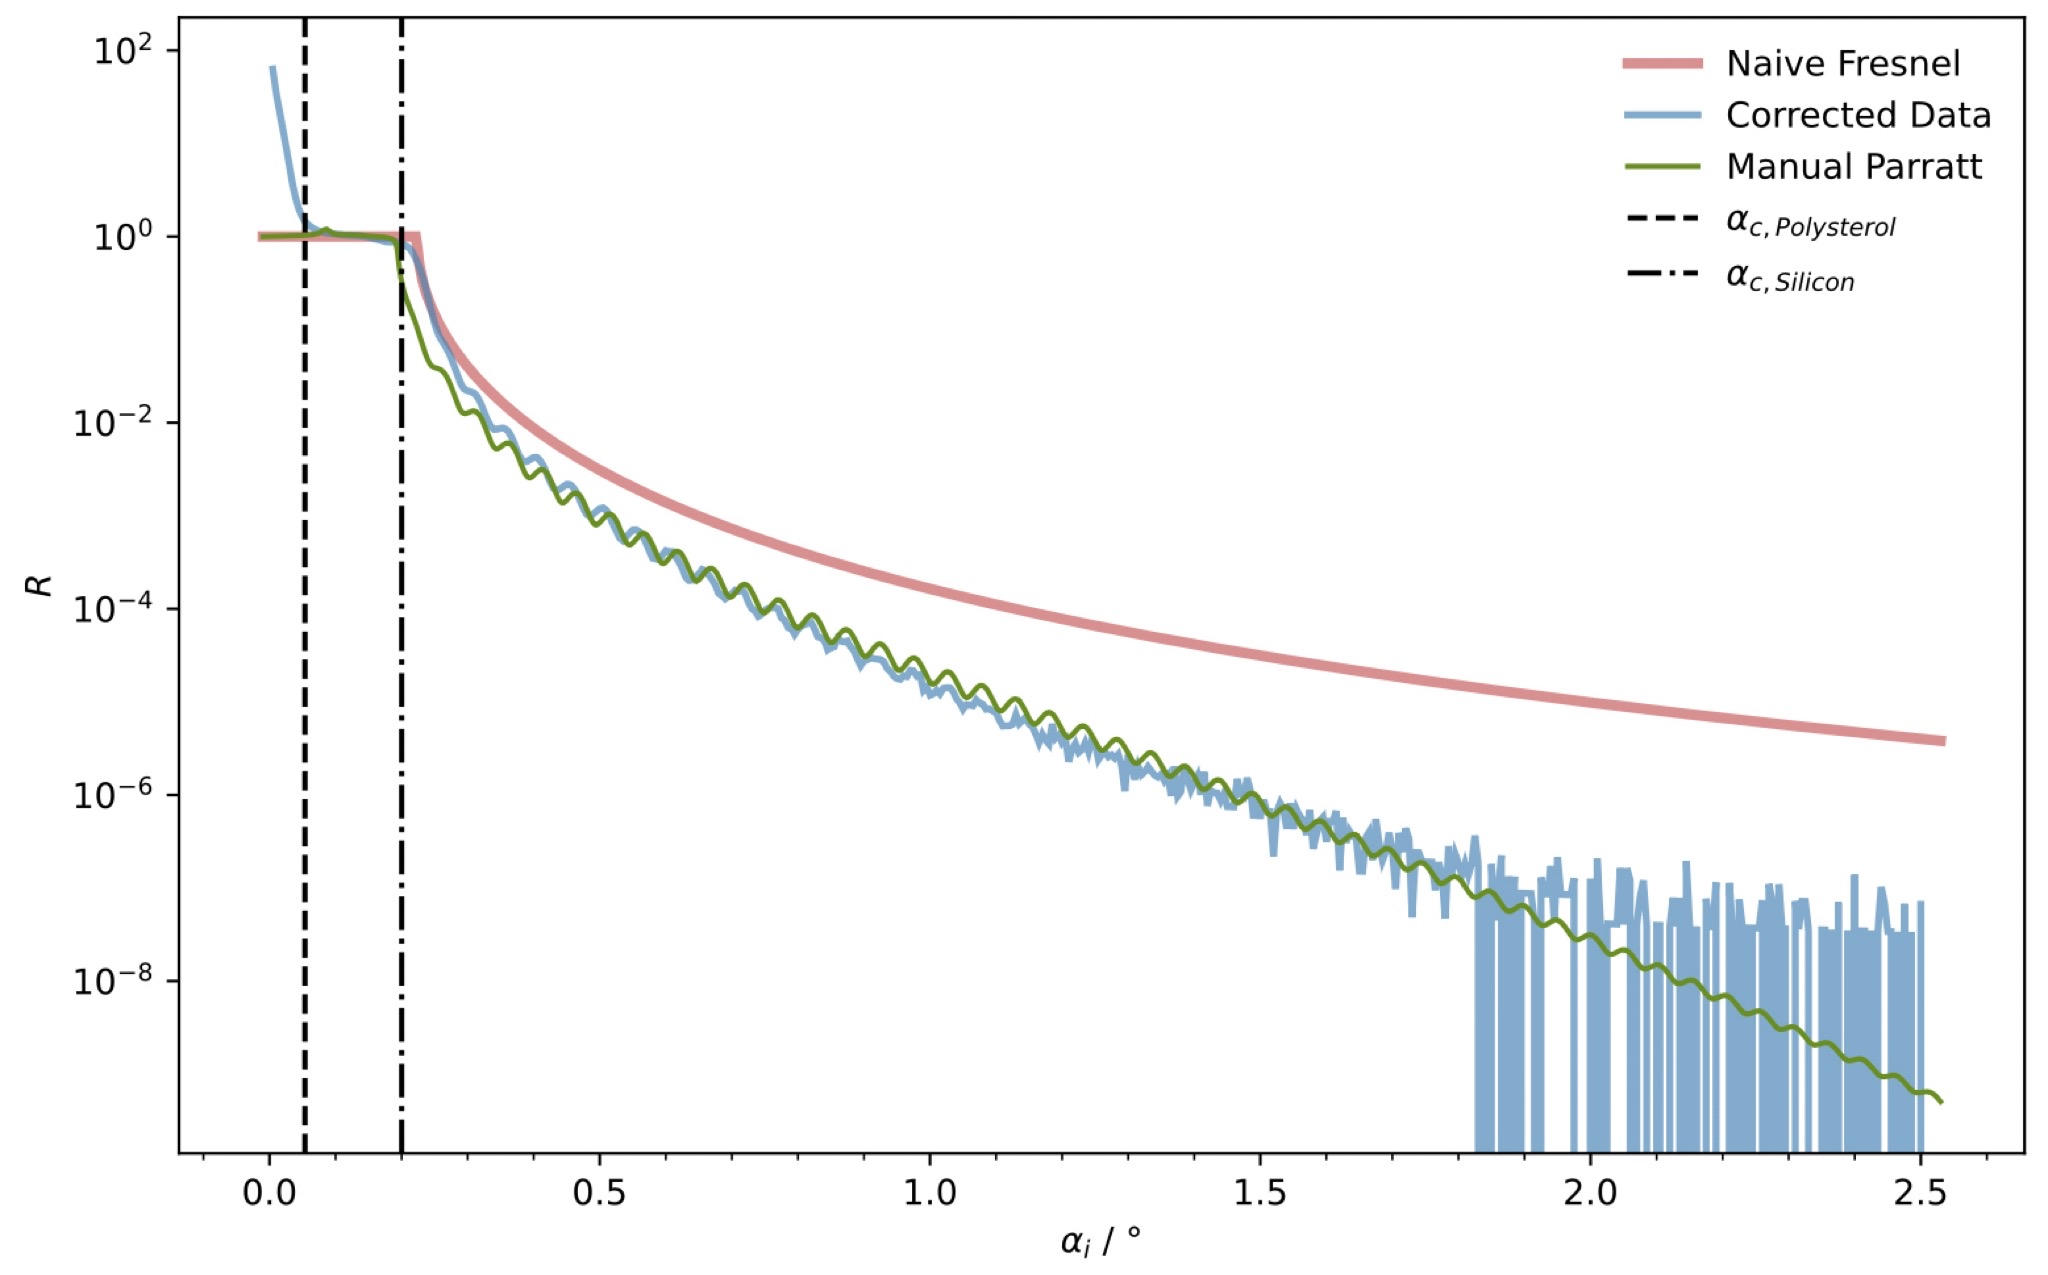
\includegraphics[width=0.88\textwidth]{content/plots/8.jpg}
	\caption{Full reflectivity curve with Parratt and Fresnel fits.}
	\label{fig:parratt-fresnel}
\end{figure}
